%%
%% This is file `hustreport-zh-example.tex',
%% generated with the docstrip utility.
%%
%% The original source files were:
%%
%% hustreport.dtx  (with options: `example-zh')
%% 
%% This is a generated file.
%% 
%% Copyright (C) 2013-2014 by Xu Cheng <xucheng@me.com>
%%               2014-2016 by hust-latex <https://github.com/hust-latex>
%% 
%% This work may be distributed and/or modified under the
%% conditions of the LaTeX Project Public License, either version 1.3
%% of this license or (at your option) any later version.
%% The latest version of this license is in
%%   http://www.latex-project.org/lppl.txt
%% and version 1.3 or later is part of all distributions of LaTeX
%% version 2005/12/01 or later.
%% 
%% This work has the LPPL maintenance status `maintained'.
%% 
%% The Current Maintainer of this work is hust-latex Organization.
%% 
%% This work consists of the files hustreport.dtx,
%% hustreport.ins and the derived file hustreport.cls
%% along with its document and example files.
%% 
%% \CharacterTable
%% {Upper-case    \A\B\C\D\E\F\G\H\I\J\K\L\M\N\O\P\Q\R\S\T\U\V\W\X\Y\Z
%%  Lower-case    \a\b\c\d\e\f\g\h\i\j\k\l\m\n\o\p\q\r\s\t\u\v\w\x\y\z
%%  Digits        \0\1\2\3\4\5\6\7\8\9
%%  Exclamation   \!     Double quote  \"     Hash (number) \#
%%  Dollar        \$     Percent       \%     Ampersand     \&
%%  Acute accent  \'     Left paren    \(     Right paren   \)
%%  Asterisk      \*     Plus          \+     Comma         \,
%%  Minus         \-     Point         \.     Solidus       \/
%%  Colon         \:     Semicolon     \;     Less than     \<
%%  Equals        \=     Greater than  \>     Question mark \?
%%  Commercial at \@     Left bracket  \[     Backslash     \\
%%  Right bracket \]     Circumflex    \^     Underscore    \_
%%  Grave accent  \`     Left brace    \{     Vertical bar  \|
%%  Right brace   \}     Tilde         \~}
\documentclass[format=draft,language=chinese,category=academic-report]{hustreport}

\usepackage{booktabs}
\usepackage{tabularx}

\graphicspath{ {./figures/} }

\stuno{1048799575}
\title{个人简历与代表性研究成果}
\author{张心泽}
\major{商务智能与电子商务}

\advisor{蔡淑琴\hspace{1em}教授}
\mentor{鲍玉昆\hspace{1em}教授}

\abstract{
    本人系管理学院15级硕士研究生,在研究生阶段一直从事基金项目、大数据实验室建设和教学助理的科研教学实践工作。
    在科研方面,本人学术兴趣广泛、热爱学习、善于思考,钻研精神强。
    在参与导师蔡淑琴教授的国家自然科学基金面上项目研究中,
    本人提出并实现了一种考虑抱怨问题路径的网络抱怨问题识别方法和基于支持向量机的在线负面口碑处理专家识别方法。
    基于其多学科交叉的知识背景,
    硕士学位论文选取了人工智能与会计账务处理的交叉研究选题,
    运用有记忆和注意力机制的循环神经网络模型实现了会计分录智能编制。
    其中,硕士学位论文已定稿答辩并将单独陈述,因此本文将主要展示网络抱怨问题识别方法与在线负面口碑处理专家识别方法。
    
    处理抱怨是企业管理活动中一项常见且重要的工作。
    本文考虑抱怨目标短语与触发短语核心词之间的句法关系,
    提出一种考虑抱怨问题路径的网络抱怨问题识别方法。
    该方法将句法关系表示为以触发短语核心词和目标短语为核心的抱怨问题路径,
    通过进行基于词库的目标短语识别、基于SVM的触发核心词识别和基于句法分析的抱怨问题路径抽取等步骤实现在线抱怨问题识别。
    通过对比实验验证了方法的有效性。

    针对在线负面口碑处理特点,
    本文提出了包含领域知识水平、情感状态和互动程度三种特征维度的专家用户识别方法以帮助企业处理在线负面口碑。
    该方法使用向量空间模型计算用户领域知识水平,
    通过情感词典计算用户情感状态,
    并引入互动程度特征,以此构建基于支持向量机的分类模型,实现专家识别。
    实验表明混合特征分类模型可以显著提高在线负面口碑处理专家识别的准确率和总体效果,验证了方法的有效性。

}
\keywords{抱怨目标,触发目标核心词,抱怨问题路径,在线负面口碑,支持向量机,专家识别}


\begin{document}

\frontmatter
\maketitle
\makeabstract
\tableofcontents
% \listoffigures
% \listoftables
\mainmatter



\chapter{考虑抱怨问题路径的网络抱怨问题识别方法}\label{chapter:1}
\section{引言}\label{sec:1.1}
在以客户为中心的市场环境中,争取、转变和维系客户是企业市场战略的关键。
处理好客户抱怨和客户服务恢复工作,对于维系良好的客户关系具有重要的作用。
企业的客户抱怨与客户保留有显著关系\cite{coussement2008improving}。
及时发现和处理客户抱怨是企业维系客户关系、降低负面口碑的危害以及增强企业盈利能力的重要方法,对企业提高管理效率和服务质量具有重要意义。

基于web2.0技术的社会化媒体平台克服了只有企业才能网络上发表内容的局限,为顾客发表不满意的产品或服务体验(即在线抱怨)提供了平台。
多样性的网络平台既激发了顾客发表的积极性也加速了这些网络抱怨的传播,在今天的网络上,抱怨随处可见。
对企业而言,在线抱怨虽然存在造成顾客流失和企业效益损失的负面影响,
但也能给企业提供产品或服务相关的有用信息,如提供辅助产品设计者进行旧产品改进和新产品设计的信息\cite{jin2016makes},
帮助企业了解顾客所关注产品或服务的问题以达到提高服务质量的目的。
\section{考生已取得的主要研究成果}\label{sec:1.2}
\begin{itemize}
    \item 张心泽,蔡淑琴,罗思宇. 基于支持向量机的在线负面口碑处理专家识别方法[J/OL]. 统计与决策,2017,(22):79-83.
    \item 张心泽. 账务智能处理中的会计机器代理研究[D]. 华中科技大学,2017.
\end{itemize}
\section{在线抱怨问题识别}\label{sec:1.3}
\subsection{在线抱怨问题表示结构}\label{subsection:1.3.1}

抱怨问题是抱怨内容反映的产品或服务存在问题的抽象表示,
它主要由抱怨目标、触发短语(触发核心词与相应修饰词)及抱怨问题路径组成:

(1)抱怨目标短语{\itshape Target\/}({\itshape Tar\/})。
作为抱怨目标,抱怨产品或服务及其特征是抱怨问题中抱怨情绪指向的对象,它是抱怨问题不可或缺的部分。
本文将抱怨产品或服务及其特征定义为抱怨目标短语。
如“根本就无法接受短信”中“短信”就是抱怨目标短语。

(2)触发短语{\itshape Problem-Word\/}({\itshape PW\/})。
考虑到描述抱怨产品及其特征的问题状态的触发短语缺乏固定模式,
触发短语的核心词(即描述目标短语问题状态的触发短语的核心词)被定义为触发核心词\textit{Trigger}(\textit{Tri}),
触发核心词及其词修饰该核心词的组合被定义为触发短语。
如“无法接受”是触发短语,“接受”是触发核心词,“无法”是触发核心词的相应修饰词。

(3)抱怨问题路径{\itshape Path\/}。
抱怨目标短语和不考虑修饰词的抱怨核心词的简单组合可形成抱怨问题,
但这样的简单组合忽略了两者间的句法关系(即De Saeger、Tutubalina等人的做法)。
本文将{(触发核心词,相应修饰词),抱怨目标短语}这样的句法关系定义并表示为抱怨问题路径。

根据如上描述,抱怨问题的识别可分解为抱怨目标短语的识别、触发核心词的识别及抱怨问题路径的抽取。
基于此,本文通过引入组成结构分析、依存结构分析和统计学习技术,设计出如\autoref{fig:1.1}所示的识别方法框架。

\begin{figure}[th]

\centering
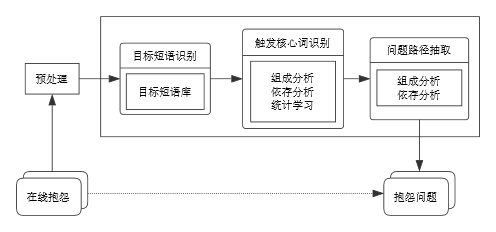
\includegraphics[width=0.9\textwidth]{figure1-1.png}
\vskip -20pt
\caption{在线抱怨问题识别框架}\label{fig:1.1}

\end{figure}

\subsection{抱怨目标短语识别}\label{subsection:1.3.2}

作为抱怨识别的一个重要组成部分,抱怨目标短语识别是后续触发核心词识别和抱怨问题路径抽取的基础。
通常情况下,抱怨目标短语指的是在线抱怨涉及的产品或服务及特征,其中产品特征又分为显性产品特征和隐性产品特征。
显性产品特征即直接出现在产品句子中的产品特征,如“这里信号好差”中的“信号”即为显性产品特征;
隐性产品特征即没有直接出现在句子里、以其他词语描述的间接方式出现的产品特征,
如“啥都没干就用了100M”中的“100M”所描述的手机流量即为隐性产品特征。

在意见挖掘领域,众多学者
(如Kurihara和Shimada\cite{kurihara2015trouble}、Liu等\cite{liu2005opinion}和Lee等\cite{lee2016mining})
为产品特征识别提出了很多不同的方法,
这些方法有效地实现了产品特征的自动抽取,然而它们需要大量难以直接获得的标记数据,且较难直接应用于其他领域。
本文通过搜索领域常用产品及其特征描述的词汇构建抱怨目标短语库,
并根据是否与所建短语库匹配的方式完成抱怨目标短语的识别。

\subsection{触发核心词识别}\label{subsection:1.3.3}
作为抱怨问题识别的关键,触发核心词的识别在抱怨问题识别中具有承上启下的作用,
一则因为触发核心词的存在与抱怨目标相对应,二则触发核心词及相应修饰词是抱怨问题路径抽取的基础。

在触发核心词识别过程中,如何确保抱怨目标短语与所识别的触发核心词相对应是一个不可回避的问题。
为解决这一问题,先将在线抱怨内容分句,进行组成结构分析,以确保抱怨目标短语和触发核心词在同一个句子中;
接着,在进行句法依存分析时,只将句子中与抱怨目标短语存在依存关系的词语作为候选触发核心词,
其他词语不予考虑。在进行这样的预处理后,可作如下假设:

\begin{assumption}\label{assumption:1.1}
    抱怨目标短语和触发核心词在同一个句子中。
\end{assumption}

\begin{assumption}\label{assumption:1.2}
    在句法分析中,触发核心词必须与抱怨目标短语存在依存关系。
\end{assumption}

基于上述假设,可将与抱怨目标短语在同一个句子且存在依存关系的词语确定为候选触发核心词,
再将触发核心词的识别转化为一个二分类问题,并训练一个有监督的高斯核支持向量机(SVM)分类器进行分类。
SVM分类器通过学习触发核心词的特征,
以判定候选触发核心词是否为既定抱怨目标短语对应的触发核心词,从而完成触发核心词的识别。

SVM是Vapnik等\cite{cortes1995support}在统计学习理论基础上提出的有监督的机器学习模型,
它被广泛应用于分类、回归分析及模式识别。
对于二分类,SVM主要通过核函数把原始空间数据向高维特征空间映射,以解决低维空间中线性不可分的问题。
具体地,设$T=\{(x_1,y_1 ),(x_2,y_2 ),\ldots,(x_n,y_n )\}$为训练数据集,
其中$x_i \in X=\mathbb R^N$,\/$y_i \in Y=\{-1,1\}(i=1,2,\ldots,N)$。
若存在向量$\bm w_i$和标量$b$,满足Mercer定理的半正定高斯核函数$K$:
\begin{equation}
    K(x_i,y_i )= \exp(- \frac{\| x_i - y_i \|}{2\delta ^2}) \label{eq:1.1}
\end{equation}

且通过$K$的数据$x_i$从原始输入空间$X$到高维特征空间$F$的映射$\phi(x_i)$满足:
\begin{equation}\label{eq:1.2}
    \begin{cases}
        \boldsymbol{w}^T_i \cdot \phi(x_i) + b \geq 0, & y_i =1 \\
        \boldsymbol{w}^T_i \cdot \phi(x_i) + b < 0, & y_i =-1 
    \end{cases}
\end{equation}

且将分类函数$f(x)$定义为:
\begin{equation}\label{eq:1.3}
    f(x_i) = \boldsymbol{W}^T_i \cdot \phi(x_i) + b
\end{equation}

通过引入松弛变量$\xi_i$和惩罚参数$C$,SVM的最大间隔分类函数可表示为:
\begin{equation}\label{eq:1.4}
    \max \frac{2}{(\| \boldsymbol{w} \| + 2C \sum^N_{i=1} \xi_i)}
\end{equation}

其中$\xi_i \geq 0$且$ y_i (\boldsymbol{w}^T_i \cdot \phi(x_i) + b) \geq 1-\xi_i$。

引入拉格朗日乘子$C \geq \alpha_i \geq 0,i=1,2,3,\ldots,n$,
根据Karush-Kuhn-Tucke条件,将求解\autoref{eq:1.4}最大间隔问题转化为使目标函数$L(\alpha_i)$最大问题:
\begin{equation}\label{eq:1.5}
    \begin{cases}
        \sum^n_{i=1} \alpha_i y_i =0, \alpha_i \geq 0  &\\
        \max\limits_\alpha L(\alpha_i)= \sum^n_{i=1} \alpha_i - \frac 12 \sum^n_{i=1}\sum^n_{j=1} \alpha_i \alpha_j y_i y_j \langle\phi(x_i),\phi(x_j)\rangle & 
    \end{cases}
\end{equation}

最后,通过序列最小最优化SMO算法对拉格朗日乘子$\alpha_i$求解,可解出$\boldsymbol{w}^T_i$和$b$:
\begin{equation}\label{eq:1.6}
    \begin{cases}
        \boldsymbol{w}_i = \sum^n_{i=1} \alpha_i y_i \phi(x_i) & \\
        b=-\frac{\max\limits_{i \colon y_i = -1} (\boldsymbol{w}^T_i \cdot \phi(x_i) ) + \min\limits_{i \colon y_i = 1}(\boldsymbol{w}^T_i \cdot \phi(x_i) )}{2} & 
    \end{cases}
\end{equation}

根据解出的$\boldsymbol{w}_i$和$b$可确定基于训练集$T$的分类函数$f(x)$,并将其用于测试数据的分类。

对于SVM分类特征,可通过包括组成结构分析和依存结构分析在内的句法分析和统计分析获取,
获取后的词语特征如\autoref{tab:1.1}所示。
\begin{table}[ht]
\centering
\caption{词语特征}\label{tab:1.1}
\vskip -10pt
\begin{tabularx}{\textwidth}{cX}
\toprule
特征类型 & 特征描述 \\
\midrule
位置特征$L$ & 是否是第一个词;是否是最后一个词;在句子中的现有位置;与抱怨目标的位置距离 \\
语法特征$Syn$ & 词性;是否是定词;是否是负面词;是否与否定词存在依存关系;是否与负面词存在依存关系;是否与把被让存在依存关系;与抱怨目标依存关系 \\
位置特征$Sta$ & 与抱怨目标的共现次数;在候选触发核心词库中出现的次数 \\
\bottomrule
\end{tabularx}
\end{table}

基于如上叙述,可设计如\autoref{alg:1.1}的触发核心词识别算法:

\begin{algorithm}[htb]
    \SetKwData{Left}{left}\SetKwData{This}{this}\SetKwData{Up}{up}
    \SetKwFunction{Union}{Union}\SetKwFunction{FindCompress}{FindCompress}
\caption{触发核心词识别算法}\label{alg:1.1}

\SetAlgoLined
\KwData{
    抱怨目标短语$Tar$:

    句子的依存结构树$DT=\{ DP,DR \}$;句子的组成结构树$CT=\{CP,CR\}$;

    触发核心词训练集
    $TrainS=\{trains_{L_p};trains_{Syn_p};trains_{Sta_p};R_{(Tar,dp_p )}\}(p=1,2,\ldots,P;R_{(Tar,dp_p )}=-1,1;)$;
    触发核心词测试集$TestS=\{tests_{L_q};tests_{Syn_q};tests_{Sta_q} \} (q=1,2,\ldots,Q; $
    $R_{(Tar,dp_p )}=-1,1)$
}
\KwResult{与抱怨目标Tar对应的触发核心词$Tri$}
\Begin{
    \For{$dp_i$ \textbu{in} $DP$}{
        \If{ $((dr(dp_i,Tar) \in DR) \parallel (dr(Tar,d_i ) \in DR))$ }{
        \textbu{append} $dp_i$ \KwTo $CW$ \;
        }
    }
    \For{$dp_p$ \textbu{in} $CW$}{
        \textbu{append} $\{trains_{L_p};trains_{Syn_p};trains_{Sta_p};R_{(Tar,dp_p )}\}$ \KwTo $Trains$ \textbu{from} $dp_p$ \;
    }
    \emph{\textbu{random select} $trains_q$ \textbu{in} $TrainS$}\;
    \emph{\textbu{trains} \textup{SVM} }\;
}

\end{algorithm}

在\autoref{alg:1.1}的句子依存结构树$DT=\{ DP,DR \}$中,
$DP$为$DT$的节点集合$\{ dp_i \}(i=1,2,⋯,M;dp_m \in Tar;dp_n \in Tri;1 \le m,n \le M)$,
$DR$为节点间的依存关系集合$\{ dr (dp_i,dp_k) \}(i,k=1,2,\ldots,N)$;
在组成结构树$CT=\{CP,CR\}$中,$CP$为组成结构树的节点集合$\{cp_j\}(j=1,2,\ldots,A;cp_a \in Tar;dp_b \in Tri;1 \le a,b \le A)$,
$CR$为节点间的依存关系集合$\{cr (cp_j,cp_s)\}(j,s=1,2,\ldots,B)$,
候选触发核心词集$CW=\{dp_p \}(p=1,2,\ldots,P)$;
在触发核心词训练集$TrainS$中,$trains_{L_p}$、$trains_{Syn_p}$、$trains_{Sta_p}$和$R_{(Tar,dp_p )}$
分别为训练集触发核心词$dp_p$的位置特征、语法特征、统计特征及类别标签;
在触发核心词测试集$TestS$中,$tests_{L_q}$、$tests_{Syn_q}$和$tests_{Sta_q}$
分别为测试集触发核心词$dp_q$的位置特征、语法特征、统计特征及类别标签;

\autoref{alg:1.1}的功能为既定抱怨目标短语识别对应的触发核心词,
它以句子的依存结构、组成结构、抱怨目标短语$Tar$、触发核心词训练集和测试集(输入时为空集,在中间过程附加数据)为输入,
以与抱怨目标短语对应的触发核心词为输出。首先,通过判断与给定的抱怨目标短语是否在同一语句且存在依存关系,
为该抱怨目标短语确定候选触发核心词;
其次,通过组成结构分析、依存结构分析和统计分析获取触发核心词的位置特征、语法特征和统计特征;
再次,将候选触发核心词集汇集为训练集和测试集;
最后,使用训练得到的SVM分类器对候选触发核心词进行分类,若$R_{(Tar,dp_q)}=1$,
则确定$dp_q$为与抱怨目标短语对应的触发核心词Tri,
此时抱怨问题被识别为以该触发核心词为核心的抱怨问题路径。

\subsection{抱怨问题路径抽取}\label{subsection:1.3.4}

为抱怨的核心,抱怨问题通常采用否定或负面词汇来描述抱怨目标短语的问题状况。
因此,如果抱怨目标短语存在问题状况,那么触发核心词要么是否定或负面词,
要么存在否定或负面词修饰触发核心词。相应地,如果触发核心词是否定或负面词,
或者存在否定或负面词修饰触发核心词(即存在特定的依存关系),
那么其所对应的抱怨目标短语极有可能存在问题状况。
另外,为了提高抱怨问题抽取的准确性,本文对双重否定的情况进行了过滤,如果触发核心词是否定或负面词,
且存在否定或负面词修饰该触发核心词,那么抱怨目标短语不存在问题状况。
鉴于此,做出如下假设:
\begin{assumption}\label{assumption:1.3}
    若触发核心词是否定或负面词,且不存在否定或负面词修饰该触发核心词,则抱怨目标短语存在问题状况。
\end{assumption}

\begin{assumption}\label{assumption:1.4}
    若触发核心词是非否定或负面词,但与否定词或负面词存在特定的依存关系,则抱怨目标短语存在问题状况。
\end{assumption}

\begin{assumption}\label{assumption:1.5}
    若触发核心词是否定或负面词,且与否定或负面词存在特定的依存关系,则抱怨目标短语不存在问题状况。
\end{assumption}

在确定抱怨目标短语是否存在问题状况后,如何抽取抱怨问题是接下来的工作。
当触发核心词属于否定或负面词,且不存在否定或负面词修饰该核心词时,
此时的触发核心词就是Gupta\cite{gupta2011extracting}定义的触发短语;当触发核心词属于非否定或负面词,
但与否点或负面词存在特定依存关系时,触发核心词和相应否定或负面修饰词的组合就是触发短语。

鉴于此,本节将抱怨问题表示为由抱怨目标短语、
触发核心词或及触发核心词的相应否定或负面修饰词组成的子树Sub-tree,
从而较好地考虑了三者间的句法关系。
通过判定是否存在与触发核心词存在特定依存关系的否定或负面词以及判定触发核心词是否本身是否定或负面词,
可归纳出如\autoref{fig:1.2}所示的抱怨问题路径抽取流程。

\begin{figure}[th]
    
    \centering
    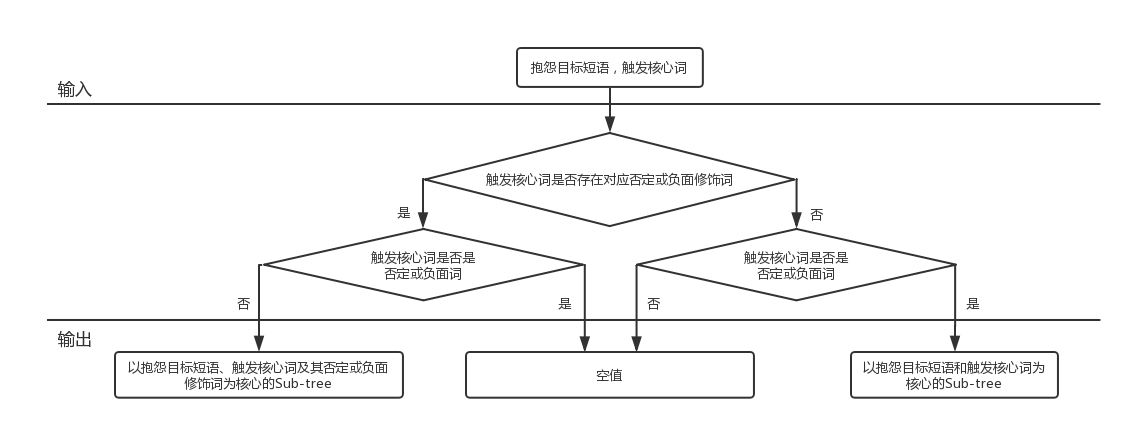
\includegraphics[width=\textwidth]{figure1-2.png}
    \vskip -20pt
    \caption{抱怨问题路径抽取流程}\label{fig:1.2}
\end{figure}

例如,“这里信号好差”中的抱怨目标短语“信号”对应的触发核心词“差”为负面词且无对应否定或负面修饰词,
因此采用由“信号”和“差”组成的Sub-tree来表示抱怨问题;
“根本就无法接受短信”中的抱怨目标短语“短信”对应的触发核心词“接受”为非负面或否定词但存在否定词“无法”对其修饰,
因此采用由“短信”、“接受”和“无法”组成的Sub-tree来表示抱怨问题。

为了更好的表述抱怨问题路径Path的生成过程,这里以在线抱怨“这里根本收不了短信!”为例详细阐述。
应用本章的抱怨目标短语识别方法和触发核心词识别方法,
可识别出本例的抱怨目标短语和触发核心词,分别为“短信”和“收”,该例的抱怨问题路径抽取过程见\autoref{fig:1.3}。

\begin{figure}[th]
    
    \centering
    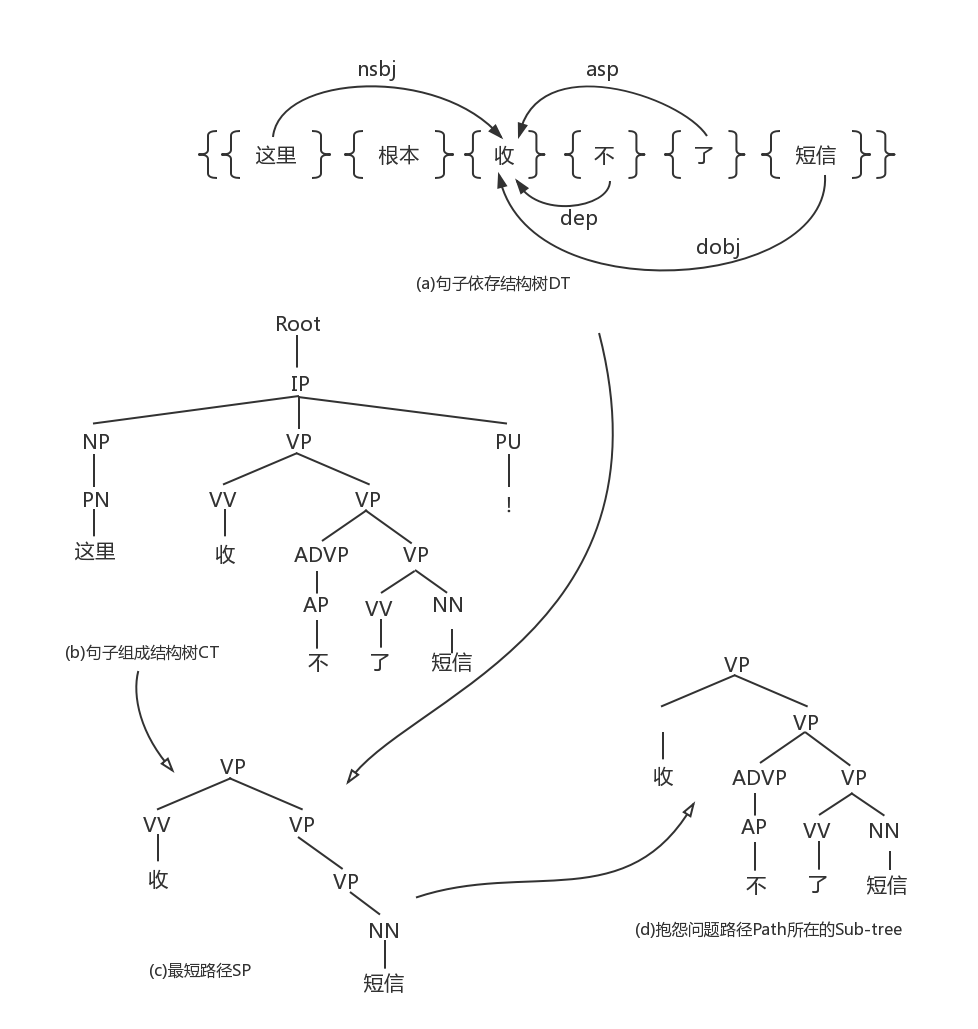
\includegraphics[width=\textwidth]{figure1-3.png}
    \vskip -20pt
    \caption{抱怨问题抽取过程}\label{fig:1.3}
\end{figure}

(1)通过Standford Parser句法分析工具,
获取如\autoref{fig:1.3}(a)和\autoref{fig:1.3}(b)所示的句子依存结构树(CT)和句法组成结构树(DT),
并获取如\autoref{fig:1.3}(c)所示的抱怨目标短语“短信”和触发核心词“收”的最短路径SP;

(2)根据\autoref{fig:1.2}的流程进行判定,可得出抱怨目标短语“短信”和触发核心词“收”外,
DP中与触发核心词“收”存在特定依存关系的有“这里”、“不”、“了”,其中只有“不”属于否定词;

(3)查找负面和否定词词库,得知触发核心词“收”即非负面也非否定词,
故将从“不”到SP根节点“VP”的路径合并到SP中,
再根据组成结构树CT可知抱怨问题路径的结构子树Sub-tree;

(4)返回抱怨问题路径抽取结果“收不了短信”。


\section{实验及结果分析}\label{sec:1.4}
\subsection{数据收集和预处理}\label{subsection:1.3.4}

为了测试抱怨问题识别方法的准确性,本文从新浪微博随机选取了281条与中国移动相关的抱怨微博作为实验数据。
由于这些数据存在相当多的噪声,在使用前需要进行一定的预处理,以消除不必要的干扰。预处理的过程如下:

(1)去除散列标签。抱怨微博文本中存在很多散列标签(如URL、“\#”、“@”),
它们又是作为句子的一部分存在,而又是只作为引用标签,
本步骤从抱怨微博文本中通过正则匹配去除无意义的散列标签,留存那些作为句子成分和陈述了抱怨问题的标签;

(2)还原简写。由于微博具有自由编辑的特性,微博用户在发表微博抱怨时可能使用简写,
如“移动”和“中移动”都是“中国移动”的简写。尽管人们可以很轻易地分析和理解这些简写,
但是实现自动地分析和理解它们不在本文讨论范畴。为处理这些简写,
本步骤通过人工构建简写还原词库,在避免歧义句的基础上(如“从中移动开”),将它们还原为“中国移动”;

(3)去除重复符号和表情符号。为了实现多样化的表达,
用户可以使用重复符号和表情符号(如“::>\_<::”)来表达特定的情绪。
由于本文主要通过语义和语法结构分析进行抱怨识别研究,
不涉及抱怨微博所需的情感信息,不需要对重复符号和表情进行分析,故在此去除重复符号和表情符号;

(4)分句分词。考虑到抱怨微博文本通常由多个句子组成,
为了保证句子组成分析和依存分析的准确性,实验对抱怨微博文本进行了分句和分词处理。

在完成了必要的预处理后,实现从281条抱怨微博中获取到了756个句子,
其中318个句子包括至少一个抱怨问题,而438个句子没有包含抱怨问题,具体的实验数据统计情况如表3所示。
\begin{table}[ht]
    \centering
    \caption{实验数据统计}\label{tab:1.3}
    \vskip -10pt
    \begin{tabularx}{\textwidth}{XY}
    \toprule
    实验数据 & 数量 \\
    \midrule
    微博数量 & 281 \\
    句子数目 & 756 \\
    微博句子平均数 & 2.69 \\
    不存在抱怨问题的句子数目 & 438 \\
    存在抱怨问题的句子数目 & 318 \\
    问题句子涉及抱怨目标短语数目 & 735 \\
    问题句子设计候选触发核心词数目 & 1363 \\
    \bottomrule
    \end{tabularx}
\end{table}

实验以318个至少包含一个抱怨问题的句子为输入,
通过完成触发目标短语识别、触发核心词识别和抱怨问题路径的抽取三个任务实现抱怨问题的识别。
在触发核心词识别实验中,实验通过句法分析从318个句子中获取1363个与抱怨目标短语存在依存关系的词语,
其中249个句子中的1040个词语作为训练集,69个句子中的323个词语作为测试集。为评价\autoref{alg:1.1},
实验基于现有的知识库信息和专家意见,采用内容编码的方式对实验数据进行了触发核心词和抱怨问题的标注。

\subsection{实验设计和评价指标}\label{subsection:1.4.2}

实验将触发核心词的识别问题转化为分类问题,并选用LibSVM包完成分类任务。
在进行抱怨问题路径抽取和触发核心词识别实验之前,
先构建描述抱怨产品及特征的词库,并基于该词库进行抱怨目标短语识别。

实验中,负面和否定词词库一部分是根据HowNet提供的3116个中文负面情感词语和1254个负面评价词语构建,
另一部分是通过收集如“不”、“没”等常用否定词构建;
此外,根据移动通信行业特征对词库进行了扩充,增加了如“慢”、“断”、“篡改”和“偷偷”之类的词语。

在抱怨问题的抽取中,句法分析以识别的抱怨目标短语及其对应触发核心词为核心,
获取满足特定条件的抱怨目标短语和触发核心词所在的组成分析树,以实现抱怨问题的抽取。

在触发核心词识别实验中,先通过Standard Parser进行句法分析,获取与抱怨目标短语存在依存关系的词语,
将这些词作为候选触发核心词,再根据句法分析、否定和负面词库获取核心词的位置特征
($Tri_L$)、语法特征($Tri_Syn$)和统计特征($Tri_Sta$),
实验通过这三类特征的7种不同组合
$Tri_L$、$Tri_Syn$、$Tri_Sta$、$Tri_{L\&Syn}$、$Tri_{L\&Sta}$、$Tri_{Syn\&Sta}$和$Tri_{L\&Syn\&Sta}$
实现触发核心词的分类,并通过结果分析选取效果最好的组合。

关于评价指标,实验采用标准机器学习分类评价指标(准确率、精确率、召回率和$F_1$值)\cite{cortes1995support}对抱怨问题的抽取和触发核心词的识别进行评价。
准确率$A$是对总体识别效果进行评价,通过识别结果中正确识别的个体与所有个体的比值来计算;
精确率$P$表示识别方法(识别触发核心词和抱怨问题)的精确性,它通过正确识别为某类别的个体数量$TP$与被识别为该类别的个体总数的比值来计算;
召回率$R$表示识别方法的完整性,它通过正确识别为某类别的个体数量$TP$与该类别下个体总数的比值来计算;
$F_1$值是精确率和召回率的调和平均值。各评价指标的具体公式如下:
\begin{align}
    A &=(TP+TN)/(TP+TN+FP+FN)\\ 
    P &=TP/(TP+FP)\\
    R &=TP/(TP+FN)\\
    F_1 &=(2PR)/(P+R)
\end{align}

本实验中,$TP$表示正确识别出的触发核心词总数;
$TN$表示正确识别出的非触发核心词总数;
$FP$表示不能构成触发核心词却被识别为触发核心词的总数;
$FN$表示可以构成触发核心词却被识别为非触发核心词的总数。


\subsection{实验结果和分析}\label{subsection:1.4.3}
根据上述实验设计和评价指标设定,触发核心词识别实验的结果如\autoref{tab:1.4}所示。
\begin{table}[ht]
    \centering
    \caption{触发核心词识别实验结果及对比}\label{tab:1.4}
    \vskip -10pt
    \begin{tabularx}{\textwidth}{lYYYYYYY}
    \toprule
    算法 & $Tri_L$ & $Tri_{Syn}$ & $Tri_{Sta}$ & $Tri_{L\&Syn}$ & $Tri_{L\&Sta}$ & $Tri_{Syn\&Sta}$ & $Tri_{L\&Syn\&Sta}$ \\
    \midrule
    准确率 & 0.7492 & 0.8824 & 0.7802 & 0.8142 & 0.7957 & 0.7956 & 0.8111 \\
    精确率 & 0 & 0.8644 & 0.6190 & 0.7839 & 0.7143 & 0.6667 & 0.7500 \\
    召回率 & 0 & 0.6296 & 0.3210 & 0.3580 & 0.3086 & 0.3704 & 0.3704 \\
    $F_1$ & 0 & 0.7286 & 0.4228 & 0.4915 & 0.4130 & 0.4762 & 0.4959 \\
    \bottomrule
    \end{tabularx}
\end{table}

由\autoref{tab:1.4}可知,在触发核心词的识别实验中只考虑语法特征的触发核心词$Tri_{Syn}$分类模型效果最佳,
这说明了模型$Tri_{Syn}$在触发核心词识别中具有明显优势。
在单类特征模型中,$Tri_{Syn}$效果最佳,$Tri_{Sta}$次之,$Tri_L$最差;
在多类特征模型中,考虑位置特征、语法特征和统计特征的$Tri_{L\&Syn\&Sta}$的效果最佳,
但与$Tri_{L\&Syn}$、$Tri_{L\&Sta}$、$Tri_{Syn\&Sta}$的效果相差不大,
且四个多类模型的触发核心词识别效果皆优于单类特征模型$Tri_L$和$Tri_{Syn}$但皆劣于$Tri_{Syn}$,
这说明语法特征能够显著提高触发核心词的识别效果,尽管位置特征和统计特征也可以用于触发核心词的识别,
但其效果明显低于语法特征。基于上述触发核心词识别实验结果对比,
实验采用效率最高的模型$Tri_{Syn}$进行触发核心词的识别,
并基于抱怨目标短语和识别的触发核心词进行抱怨问题路径抽取,进而完成对抱怨问题的识别。

综上所述,本文进行的实验有如下发现:语法特征对提高抱怨问题触发核心词识别的准确性具有显著作用;
抱怨目标短语和抱怨问题触发核心词的简单组合不能很好地表示抱怨问题,考虑两者的句法关系可以提高抱怨问题识别的准确性。
\section{结论}\label{sec:1.5}
本文提出了一种考虑抱怨问题路径的在线抱怨问题识别方法,
该方法采用抱怨问题路径的方式表示抱怨目标短语和触发短语核心词之间的句法关系,
先后通过识别抱怨目标短语、识别触发核心词和抽取抱怨问题路径,实现在线抱怨问题的自动识别。
为测试方法的准确性和有效性,本文进行了对比实验,
实验结果表明考虑抱怨目标短语和触发核心词间的句法关系可以提高抱怨问题识别的准确性。

在接下来的研究中,将增加实验数据的多样性,以提高所提方法的泛化能力;
另外,方法中触发核心词的识别与抱怨问题的抽取均基于句法分析,由于中文的复杂性,
错误的句法分析会直接影响到方法的准确性,因此研究提高中文句法分析的效果也是未来工作之一。
\chapter{考虑抱怨问题路径的网络抱怨问题识别方法}\label{chapter:1}
\section{引言}\label{sec:1.1}
在以客户为中心的市场环境中,争取、转变和维系客户是企业市场战略的关键。
处理好客户抱怨和客户服务恢复工作,对于维系良好的客户关系具有重要的作用。
企业的客户抱怨与客户保留有显著关系\cite{coussement2008improving}。
及时发现和处理客户抱怨是企业维系客户关系、降低负面口碑的危害以及增强企业盈利能力的重要方法,对企业提高管理效率和服务质量具有重要意义。

基于web2.0技术的社会化媒体平台克服了只有企业才能网络上发表内容的局限,为顾客发表不满意的产品或服务体验(即在线抱怨)提供了平台。
多样性的网络平台既激发了顾客发表的积极性也加速了这些网络抱怨的传播,在今天的网络上,抱怨随处可见。
对企业而言,在线抱怨虽然存在造成顾客流失和企业效益损失的负面影响,
但也能给企业提供产品或服务相关的有用信息,如提供辅助产品设计者进行旧产品改进和新产品设计的信息\cite{jin2016makes},
帮助企业了解顾客所关注产品或服务的问题以达到提高服务质量的目的。
\section{考生已取得的主要研究成果}\label{sec:1.2}
\begin{itemize}
    \item 张心泽,蔡淑琴,罗思宇. 基于支持向量机的在线负面口碑处理专家识别方法[J/OL]. 统计与决策,2017,(22):79-83.
    \item 张心泽. 账务智能处理中的会计机器代理研究[D]. 华中科技大学,2017.
\end{itemize}
\section{在线抱怨问题识别}\label{sec:1.3}
\subsection{在线抱怨问题表示结构}\label{subsection:1.3.1}

抱怨问题是抱怨内容反映的产品或服务存在问题的抽象表示,
它主要由抱怨目标、触发短语(触发核心词与相应修饰词)及抱怨问题路径组成:

(1)抱怨目标短语{\itshape Target\/}({\itshape Tar\/})。
作为抱怨目标,抱怨产品或服务及其特征是抱怨问题中抱怨情绪指向的对象,它是抱怨问题不可或缺的部分。
本文将抱怨产品或服务及其特征定义为抱怨目标短语。
如“根本就无法接受短信”中“短信”就是抱怨目标短语。

(2)触发短语{\itshape Problem-Word\/}({\itshape PW\/})。
考虑到描述抱怨产品及其特征的问题状态的触发短语缺乏固定模式,
触发短语的核心词(即描述目标短语问题状态的触发短语的核心词)被定义为触发核心词\textit{Trigger}(\textit{Tri}),
触发核心词及其词修饰该核心词的组合被定义为触发短语。
如“无法接受”是触发短语,“接受”是触发核心词,“无法”是触发核心词的相应修饰词。

(3)抱怨问题路径{\itshape Path\/}。
抱怨目标短语和不考虑修饰词的抱怨核心词的简单组合可形成抱怨问题,
但这样的简单组合忽略了两者间的句法关系(即De Saeger、Tutubalina等人的做法)。
本文将{(触发核心词,相应修饰词),抱怨目标短语}这样的句法关系定义并表示为抱怨问题路径。

根据如上描述,抱怨问题的识别可分解为抱怨目标短语的识别、触发核心词的识别及抱怨问题路径的抽取。
基于此,本文通过引入组成结构分析、依存结构分析和统计学习技术,设计出如\autoref{fig:1.1}所示的识别方法框架。

\begin{figure}[th]

\centering
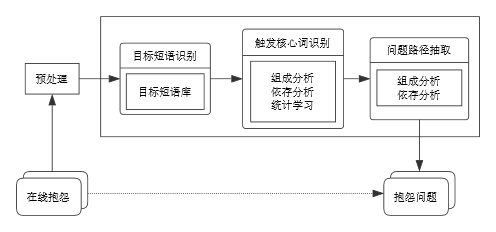
\includegraphics[width=0.9\textwidth]{figure1-1.png}
\vskip -20pt
\caption{在线抱怨问题识别框架}\label{fig:1.1}

\end{figure}

\subsection{抱怨目标短语识别}\label{subsection:1.3.2}

作为抱怨识别的一个重要组成部分,抱怨目标短语识别是后续触发核心词识别和抱怨问题路径抽取的基础。
通常情况下,抱怨目标短语指的是在线抱怨涉及的产品或服务及特征,其中产品特征又分为显性产品特征和隐性产品特征。
显性产品特征即直接出现在产品句子中的产品特征,如“这里信号好差”中的“信号”即为显性产品特征;
隐性产品特征即没有直接出现在句子里、以其他词语描述的间接方式出现的产品特征,
如“啥都没干就用了100M”中的“100M”所描述的手机流量即为隐性产品特征。

在意见挖掘领域,众多学者
(如Kurihara和Shimada\cite{kurihara2015trouble}、Liu等\cite{liu2005opinion}和Lee等\cite{lee2016mining})
为产品特征识别提出了很多不同的方法,
这些方法有效地实现了产品特征的自动抽取,然而它们需要大量难以直接获得的标记数据,且较难直接应用于其他领域。
本文通过搜索领域常用产品及其特征描述的词汇构建抱怨目标短语库,
并根据是否与所建短语库匹配的方式完成抱怨目标短语的识别。

\subsection{触发核心词识别}\label{subsection:1.3.3}
作为抱怨问题识别的关键,触发核心词的识别在抱怨问题识别中具有承上启下的作用,
一则因为触发核心词的存在与抱怨目标相对应,二则触发核心词及相应修饰词是抱怨问题路径抽取的基础。

在触发核心词识别过程中,如何确保抱怨目标短语与所识别的触发核心词相对应是一个不可回避的问题。
为解决这一问题,先将在线抱怨内容分句,进行组成结构分析,以确保抱怨目标短语和触发核心词在同一个句子中;
接着,在进行句法依存分析时,只将句子中与抱怨目标短语存在依存关系的词语作为候选触发核心词,
其他词语不予考虑。在进行这样的预处理后,可作如下假设:

\begin{assumption}\label{assumption:1.1}
    抱怨目标短语和触发核心词在同一个句子中。
\end{assumption}

\begin{assumption}\label{assumption:1.2}
    在句法分析中,触发核心词必须与抱怨目标短语存在依存关系。
\end{assumption}

基于上述假设,可将与抱怨目标短语在同一个句子且存在依存关系的词语确定为候选触发核心词,
再将触发核心词的识别转化为一个二分类问题,并训练一个有监督的高斯核支持向量机(SVM)分类器进行分类。
SVM分类器通过学习触发核心词的特征,
以判定候选触发核心词是否为既定抱怨目标短语对应的触发核心词,从而完成触发核心词的识别。

SVM是Vapnik等\cite{cortes1995support}在统计学习理论基础上提出的有监督的机器学习模型,
它被广泛应用于分类、回归分析及模式识别。
对于二分类,SVM主要通过核函数把原始空间数据向高维特征空间映射,以解决低维空间中线性不可分的问题。
具体地,设$T=\{(x_1,y_1 ),(x_2,y_2 ),\ldots,(x_n,y_n )\}$为训练数据集,
其中$x_i \in X=\mathbb R^N$,\/$y_i \in Y=\{-1,1\}(i=1,2,\ldots,N)$。
若存在向量$\bm w_i$和标量$b$,满足Mercer定理的半正定高斯核函数$K$:
\begin{equation}
    K(x_i,y_i )= \exp(- \frac{\| x_i - y_i \|}{2\delta ^2}) \label{eq:1.1}
\end{equation}

且通过$K$的数据$x_i$从原始输入空间$X$到高维特征空间$F$的映射$\phi(x_i)$满足:
\begin{equation}\label{eq:1.2}
    \begin{cases}
        \boldsymbol{w}^T_i \cdot \phi(x_i) + b \geq 0, & y_i =1 \\
        \boldsymbol{w}^T_i \cdot \phi(x_i) + b < 0, & y_i =-1 
    \end{cases}
\end{equation}

且将分类函数$f(x)$定义为:
\begin{equation}\label{eq:1.3}
    f(x_i) = \boldsymbol{W}^T_i \cdot \phi(x_i) + b
\end{equation}

通过引入松弛变量$\xi_i$和惩罚参数$C$,SVM的最大间隔分类函数可表示为:
\begin{equation}\label{eq:1.4}
    \max \frac{2}{(\| \boldsymbol{w} \| + 2C \sum^N_{i=1} \xi_i)}
\end{equation}

其中$\xi_i \geq 0$且$ y_i (\boldsymbol{w}^T_i \cdot \phi(x_i) + b) \geq 1-\xi_i$。

引入拉格朗日乘子$C \geq \alpha_i \geq 0,i=1,2,3,\ldots,n$,
根据Karush-Kuhn-Tucke条件,将求解\autoref{eq:1.4}最大间隔问题转化为使目标函数$L(\alpha_i)$最大问题:
\begin{equation}\label{eq:1.5}
    \begin{cases}
        \sum^n_{i=1} \alpha_i y_i =0, \alpha_i \geq 0  &\\
        \max\limits_\alpha L(\alpha_i)= \sum^n_{i=1} \alpha_i - \frac 12 \sum^n_{i=1}\sum^n_{j=1} \alpha_i \alpha_j y_i y_j \langle\phi(x_i),\phi(x_j)\rangle & 
    \end{cases}
\end{equation}

最后,通过序列最小最优化SMO算法对拉格朗日乘子$\alpha_i$求解,可解出$\boldsymbol{w}^T_i$和$b$:
\begin{equation}\label{eq:1.6}
    \begin{cases}
        \boldsymbol{w}_i = \sum^n_{i=1} \alpha_i y_i \phi(x_i) & \\
        b=-\frac{\max\limits_{i \colon y_i = -1} (\boldsymbol{w}^T_i \cdot \phi(x_i) ) + \min\limits_{i \colon y_i = 1}(\boldsymbol{w}^T_i \cdot \phi(x_i) )}{2} & 
    \end{cases}
\end{equation}

根据解出的$\boldsymbol{w}_i$和$b$可确定基于训练集$T$的分类函数$f(x)$,并将其用于测试数据的分类。

对于SVM分类特征,可通过包括组成结构分析和依存结构分析在内的句法分析和统计分析获取,
获取后的词语特征如\autoref{tab:1.1}所示。
\begin{table}[ht]
\centering
\caption{词语特征}\label{tab:1.1}
\vskip -10pt
\begin{tabularx}{\textwidth}{cX}
\toprule
特征类型 & 特征描述 \\
\midrule
位置特征$L$ & 是否是第一个词;是否是最后一个词;在句子中的现有位置;与抱怨目标的位置距离 \\
语法特征$Syn$ & 词性;是否是定词;是否是负面词;是否与否定词存在依存关系;是否与负面词存在依存关系;是否与把被让存在依存关系;与抱怨目标依存关系 \\
位置特征$Sta$ & 与抱怨目标的共现次数;在候选触发核心词库中出现的次数 \\
\bottomrule
\end{tabularx}
\end{table}

基于如上叙述,可设计如\autoref{alg:1.1}的触发核心词识别算法:

\begin{algorithm}[htb]
    \SetKwData{Left}{left}\SetKwData{This}{this}\SetKwData{Up}{up}
    \SetKwFunction{Union}{Union}\SetKwFunction{FindCompress}{FindCompress}
\caption{触发核心词识别算法}\label{alg:1.1}

\SetAlgoLined
\KwData{
    抱怨目标短语$Tar$:

    句子的依存结构树$DT=\{ DP,DR \}$;句子的组成结构树$CT=\{CP,CR\}$;

    触发核心词训练集
    $TrainS=\{trains_{L_p};trains_{Syn_p};trains_{Sta_p};R_{(Tar,dp_p )}\}(p=1,2,\ldots,P;R_{(Tar,dp_p )}=-1,1;)$;
    触发核心词测试集$TestS=\{tests_{L_q};tests_{Syn_q};tests_{Sta_q} \} (q=1,2,\ldots,Q; $
    $R_{(Tar,dp_p )}=-1,1)$
}
\KwResult{与抱怨目标Tar对应的触发核心词$Tri$}
\Begin{
    \For{$dp_i$ \textbu{in} $DP$}{
        \If{ $((dr(dp_i,Tar) \in DR) \parallel (dr(Tar,d_i ) \in DR))$ }{
        \textbu{append} $dp_i$ \KwTo $CW$ \;
        }
    }
    \For{$dp_p$ \textbu{in} $CW$}{
        \textbu{append} $\{trains_{L_p};trains_{Syn_p};trains_{Sta_p};R_{(Tar,dp_p )}\}$ \KwTo $Trains$ \textbu{from} $dp_p$ \;
    }
    \emph{\textbu{random select} $trains_q$ \textbu{in} $TrainS$}\;
    \emph{\textbu{trains} \textup{SVM} }\;
}

\end{algorithm}

在\autoref{alg:1.1}的句子依存结构树$DT=\{ DP,DR \}$中,
$DP$为$DT$的节点集合$\{ dp_i \}(i=1,2,⋯,M;dp_m \in Tar;dp_n \in Tri;1 \le m,n \le M)$,
$DR$为节点间的依存关系集合$\{ dr (dp_i,dp_k) \}(i,k=1,2,\ldots,N)$;
在组成结构树$CT=\{CP,CR\}$中,$CP$为组成结构树的节点集合$\{cp_j\}(j=1,2,\ldots,A;cp_a \in Tar;dp_b \in Tri;1 \le a,b \le A)$,
$CR$为节点间的依存关系集合$\{cr (cp_j,cp_s)\}(j,s=1,2,\ldots,B)$,
候选触发核心词集$CW=\{dp_p \}(p=1,2,\ldots,P)$;
在触发核心词训练集$TrainS$中,$trains_{L_p}$、$trains_{Syn_p}$、$trains_{Sta_p}$和$R_{(Tar,dp_p )}$
分别为训练集触发核心词$dp_p$的位置特征、语法特征、统计特征及类别标签;
在触发核心词测试集$TestS$中,$tests_{L_q}$、$tests_{Syn_q}$和$tests_{Sta_q}$
分别为测试集触发核心词$dp_q$的位置特征、语法特征、统计特征及类别标签;

\autoref{alg:1.1}的功能为既定抱怨目标短语识别对应的触发核心词,
它以句子的依存结构、组成结构、抱怨目标短语$Tar$、触发核心词训练集和测试集(输入时为空集,在中间过程附加数据)为输入,
以与抱怨目标短语对应的触发核心词为输出。首先,通过判断与给定的抱怨目标短语是否在同一语句且存在依存关系,
为该抱怨目标短语确定候选触发核心词;
其次,通过组成结构分析、依存结构分析和统计分析获取触发核心词的位置特征、语法特征和统计特征;
再次,将候选触发核心词集汇集为训练集和测试集;
最后,使用训练得到的SVM分类器对候选触发核心词进行分类,若$R_{(Tar,dp_q)}=1$,
则确定$dp_q$为与抱怨目标短语对应的触发核心词Tri,
此时抱怨问题被识别为以该触发核心词为核心的抱怨问题路径。

\subsection{抱怨问题路径抽取}\label{subsection:1.3.4}

为抱怨的核心,抱怨问题通常采用否定或负面词汇来描述抱怨目标短语的问题状况。
因此,如果抱怨目标短语存在问题状况,那么触发核心词要么是否定或负面词,
要么存在否定或负面词修饰触发核心词。相应地,如果触发核心词是否定或负面词,
或者存在否定或负面词修饰触发核心词(即存在特定的依存关系),
那么其所对应的抱怨目标短语极有可能存在问题状况。
另外,为了提高抱怨问题抽取的准确性,本文对双重否定的情况进行了过滤,如果触发核心词是否定或负面词,
且存在否定或负面词修饰该触发核心词,那么抱怨目标短语不存在问题状况。
鉴于此,做出如下假设:
\begin{assumption}\label{assumption:1.3}
    若触发核心词是否定或负面词,且不存在否定或负面词修饰该触发核心词,则抱怨目标短语存在问题状况。
\end{assumption}

\begin{assumption}\label{assumption:1.4}
    若触发核心词是非否定或负面词,但与否定词或负面词存在特定的依存关系,则抱怨目标短语存在问题状况。
\end{assumption}

\begin{assumption}\label{assumption:1.5}
    若触发核心词是否定或负面词,且与否定或负面词存在特定的依存关系,则抱怨目标短语不存在问题状况。
\end{assumption}

在确定抱怨目标短语是否存在问题状况后,如何抽取抱怨问题是接下来的工作。
当触发核心词属于否定或负面词,且不存在否定或负面词修饰该核心词时,
此时的触发核心词就是Gupta\cite{gupta2011extracting}定义的触发短语;当触发核心词属于非否定或负面词,
但与否点或负面词存在特定依存关系时,触发核心词和相应否定或负面修饰词的组合就是触发短语。

鉴于此,本节将抱怨问题表示为由抱怨目标短语、
触发核心词或及触发核心词的相应否定或负面修饰词组成的子树Sub-tree,
从而较好地考虑了三者间的句法关系。
通过判定是否存在与触发核心词存在特定依存关系的否定或负面词以及判定触发核心词是否本身是否定或负面词,
可归纳出如\autoref{fig:1.2}所示的抱怨问题路径抽取流程。

\begin{figure}[th]
    
    \centering
    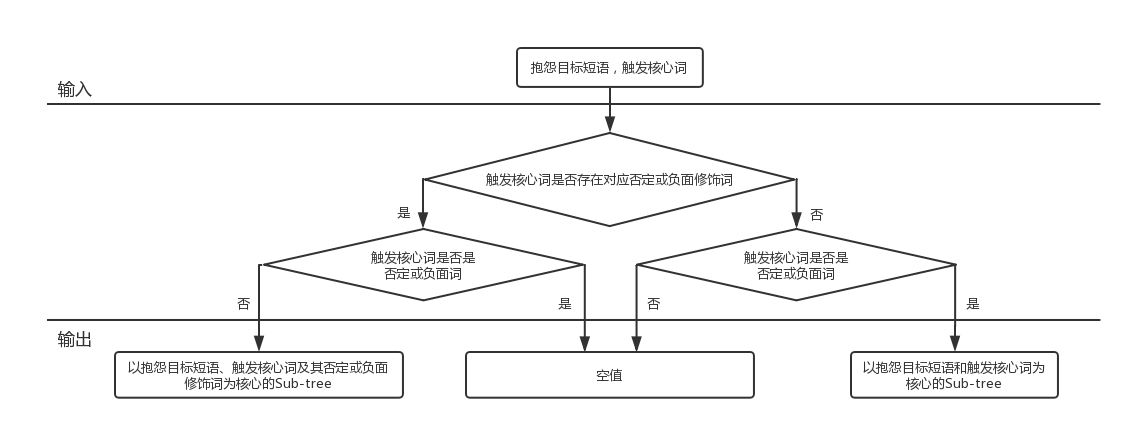
\includegraphics[width=\textwidth]{figure1-2.png}
    \vskip -20pt
    \caption{抱怨问题路径抽取流程}\label{fig:1.2}
\end{figure}

例如,“这里信号好差”中的抱怨目标短语“信号”对应的触发核心词“差”为负面词且无对应否定或负面修饰词,
因此采用由“信号”和“差”组成的Sub-tree来表示抱怨问题;
“根本就无法接受短信”中的抱怨目标短语“短信”对应的触发核心词“接受”为非负面或否定词但存在否定词“无法”对其修饰,
因此采用由“短信”、“接受”和“无法”组成的Sub-tree来表示抱怨问题。

为了更好的表述抱怨问题路径Path的生成过程,这里以在线抱怨“这里根本收不了短信!”为例详细阐述。
应用本章的抱怨目标短语识别方法和触发核心词识别方法,
可识别出本例的抱怨目标短语和触发核心词,分别为“短信”和“收”,该例的抱怨问题路径抽取过程见\autoref{fig:1.3}。

\begin{figure}[th]
    
    \centering
    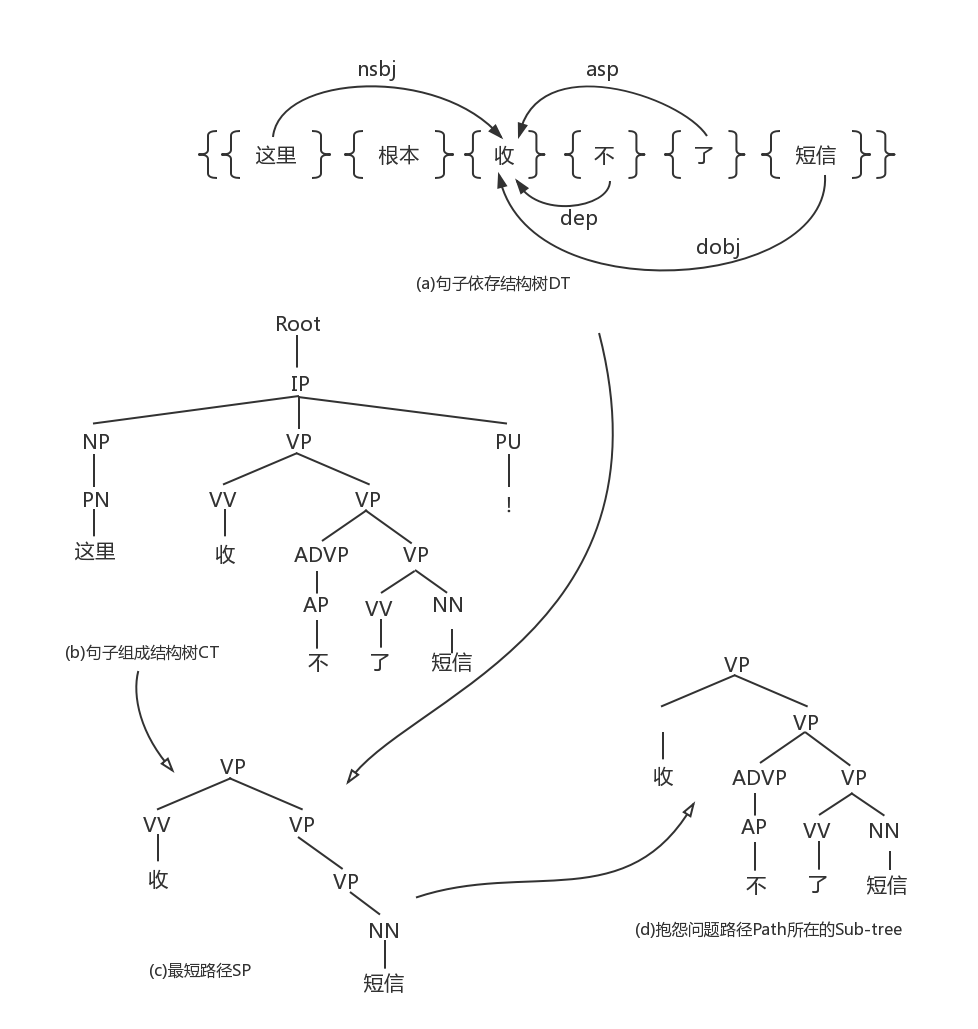
\includegraphics[width=\textwidth]{figure1-3.png}
    \vskip -20pt
    \caption{抱怨问题抽取过程}\label{fig:1.3}
\end{figure}

(1)通过Standford Parser句法分析工具,
获取如\autoref{fig:1.3}(a)和\autoref{fig:1.3}(b)所示的句子依存结构树(CT)和句法组成结构树(DT),
并获取如\autoref{fig:1.3}(c)所示的抱怨目标短语“短信”和触发核心词“收”的最短路径SP;

(2)根据\autoref{fig:1.2}的流程进行判定,可得出抱怨目标短语“短信”和触发核心词“收”外,
DP中与触发核心词“收”存在特定依存关系的有“这里”、“不”、“了”,其中只有“不”属于否定词;

(3)查找负面和否定词词库,得知触发核心词“收”即非负面也非否定词,
故将从“不”到SP根节点“VP”的路径合并到SP中,
再根据组成结构树CT可知抱怨问题路径的结构子树Sub-tree;

(4)返回抱怨问题路径抽取结果“收不了短信”。


\section{实验及结果分析}\label{sec:1.4}
\subsection{数据收集和预处理}\label{subsection:1.3.4}

为了测试抱怨问题识别方法的准确性,本文从新浪微博随机选取了281条与中国移动相关的抱怨微博作为实验数据。
由于这些数据存在相当多的噪声,在使用前需要进行一定的预处理,以消除不必要的干扰。预处理的过程如下:

(1)去除散列标签。抱怨微博文本中存在很多散列标签(如URL、“\#”、“@”),
它们又是作为句子的一部分存在,而又是只作为引用标签,
本步骤从抱怨微博文本中通过正则匹配去除无意义的散列标签,留存那些作为句子成分和陈述了抱怨问题的标签;

(2)还原简写。由于微博具有自由编辑的特性,微博用户在发表微博抱怨时可能使用简写,
如“移动”和“中移动”都是“中国移动”的简写。尽管人们可以很轻易地分析和理解这些简写,
但是实现自动地分析和理解它们不在本文讨论范畴。为处理这些简写,
本步骤通过人工构建简写还原词库,在避免歧义句的基础上(如“从中移动开”),将它们还原为“中国移动”;

(3)去除重复符号和表情符号。为了实现多样化的表达,
用户可以使用重复符号和表情符号(如“::>\_<::”)来表达特定的情绪。
由于本文主要通过语义和语法结构分析进行抱怨识别研究,
不涉及抱怨微博所需的情感信息,不需要对重复符号和表情进行分析,故在此去除重复符号和表情符号;

(4)分句分词。考虑到抱怨微博文本通常由多个句子组成,
为了保证句子组成分析和依存分析的准确性,实验对抱怨微博文本进行了分句和分词处理。

在完成了必要的预处理后,实现从281条抱怨微博中获取到了756个句子,
其中318个句子包括至少一个抱怨问题,而438个句子没有包含抱怨问题,具体的实验数据统计情况如表3所示。
\begin{table}[ht]
    \centering
    \caption{实验数据统计}\label{tab:1.3}
    \vskip -10pt
    \begin{tabularx}{\textwidth}{XY}
    \toprule
    实验数据 & 数量 \\
    \midrule
    微博数量 & 281 \\
    句子数目 & 756 \\
    微博句子平均数 & 2.69 \\
    不存在抱怨问题的句子数目 & 438 \\
    存在抱怨问题的句子数目 & 318 \\
    问题句子涉及抱怨目标短语数目 & 735 \\
    问题句子设计候选触发核心词数目 & 1363 \\
    \bottomrule
    \end{tabularx}
\end{table}

实验以318个至少包含一个抱怨问题的句子为输入,
通过完成触发目标短语识别、触发核心词识别和抱怨问题路径的抽取三个任务实现抱怨问题的识别。
在触发核心词识别实验中,实验通过句法分析从318个句子中获取1363个与抱怨目标短语存在依存关系的词语,
其中249个句子中的1040个词语作为训练集,69个句子中的323个词语作为测试集。为评价\autoref{alg:1.1},
实验基于现有的知识库信息和专家意见,采用内容编码的方式对实验数据进行了触发核心词和抱怨问题的标注。

\subsection{实验设计和评价指标}\label{subsection:1.4.2}

实验将触发核心词的识别问题转化为分类问题,并选用LibSVM包完成分类任务。
在进行抱怨问题路径抽取和触发核心词识别实验之前,
先构建描述抱怨产品及特征的词库,并基于该词库进行抱怨目标短语识别。

实验中,负面和否定词词库一部分是根据HowNet提供的3116个中文负面情感词语和1254个负面评价词语构建,
另一部分是通过收集如“不”、“没”等常用否定词构建;
此外,根据移动通信行业特征对词库进行了扩充,增加了如“慢”、“断”、“篡改”和“偷偷”之类的词语。

在抱怨问题的抽取中,句法分析以识别的抱怨目标短语及其对应触发核心词为核心,
获取满足特定条件的抱怨目标短语和触发核心词所在的组成分析树,以实现抱怨问题的抽取。

在触发核心词识别实验中,先通过Standard Parser进行句法分析,获取与抱怨目标短语存在依存关系的词语,
将这些词作为候选触发核心词,再根据句法分析、否定和负面词库获取核心词的位置特征
($Tri_L$)、语法特征($Tri_Syn$)和统计特征($Tri_Sta$),
实验通过这三类特征的7种不同组合
$Tri_L$、$Tri_Syn$、$Tri_Sta$、$Tri_{L\&Syn}$、$Tri_{L\&Sta}$、$Tri_{Syn\&Sta}$和$Tri_{L\&Syn\&Sta}$
实现触发核心词的分类,并通过结果分析选取效果最好的组合。

关于评价指标,实验采用标准机器学习分类评价指标(准确率、精确率、召回率和$F_1$值)\cite{cortes1995support}对抱怨问题的抽取和触发核心词的识别进行评价。
准确率$A$是对总体识别效果进行评价,通过识别结果中正确识别的个体与所有个体的比值来计算;
精确率$P$表示识别方法(识别触发核心词和抱怨问题)的精确性,它通过正确识别为某类别的个体数量$TP$与被识别为该类别的个体总数的比值来计算;
召回率$R$表示识别方法的完整性,它通过正确识别为某类别的个体数量$TP$与该类别下个体总数的比值来计算;
$F_1$值是精确率和召回率的调和平均值。各评价指标的具体公式如下:
\begin{align}
    A &=(TP+TN)/(TP+TN+FP+FN)\\ 
    P &=TP/(TP+FP)\\
    R &=TP/(TP+FN)\\
    F_1 &=(2PR)/(P+R)
\end{align}

本实验中,$TP$表示正确识别出的触发核心词总数;
$TN$表示正确识别出的非触发核心词总数;
$FP$表示不能构成触发核心词却被识别为触发核心词的总数;
$FN$表示可以构成触发核心词却被识别为非触发核心词的总数。


\subsection{实验结果和分析}\label{subsection:1.4.3}
根据上述实验设计和评价指标设定,触发核心词识别实验的结果如\autoref{tab:1.4}所示。
\begin{table}[ht]
    \centering
    \caption{触发核心词识别实验结果及对比}\label{tab:1.4}
    \vskip -10pt
    \begin{tabularx}{\textwidth}{lYYYYYYY}
    \toprule
    算法 & $Tri_L$ & $Tri_{Syn}$ & $Tri_{Sta}$ & $Tri_{L\&Syn}$ & $Tri_{L\&Sta}$ & $Tri_{Syn\&Sta}$ & $Tri_{L\&Syn\&Sta}$ \\
    \midrule
    准确率 & 0.7492 & 0.8824 & 0.7802 & 0.8142 & 0.7957 & 0.7956 & 0.8111 \\
    精确率 & 0 & 0.8644 & 0.6190 & 0.7839 & 0.7143 & 0.6667 & 0.7500 \\
    召回率 & 0 & 0.6296 & 0.3210 & 0.3580 & 0.3086 & 0.3704 & 0.3704 \\
    $F_1$ & 0 & 0.7286 & 0.4228 & 0.4915 & 0.4130 & 0.4762 & 0.4959 \\
    \bottomrule
    \end{tabularx}
\end{table}

由\autoref{tab:1.4}可知,在触发核心词的识别实验中只考虑语法特征的触发核心词$Tri_{Syn}$分类模型效果最佳,
这说明了模型$Tri_{Syn}$在触发核心词识别中具有明显优势。
在单类特征模型中,$Tri_{Syn}$效果最佳,$Tri_{Sta}$次之,$Tri_L$最差;
在多类特征模型中,考虑位置特征、语法特征和统计特征的$Tri_{L\&Syn\&Sta}$的效果最佳,
但与$Tri_{L\&Syn}$、$Tri_{L\&Sta}$、$Tri_{Syn\&Sta}$的效果相差不大,
且四个多类模型的触发核心词识别效果皆优于单类特征模型$Tri_L$和$Tri_{Syn}$但皆劣于$Tri_{Syn}$,
这说明语法特征能够显著提高触发核心词的识别效果,尽管位置特征和统计特征也可以用于触发核心词的识别,
但其效果明显低于语法特征。基于上述触发核心词识别实验结果对比,
实验采用效率最高的模型$Tri_{Syn}$进行触发核心词的识别,
并基于抱怨目标短语和识别的触发核心词进行抱怨问题路径抽取,进而完成对抱怨问题的识别。

综上所述,本文进行的实验有如下发现:语法特征对提高抱怨问题触发核心词识别的准确性具有显著作用;
抱怨目标短语和抱怨问题触发核心词的简单组合不能很好地表示抱怨问题,考虑两者的句法关系可以提高抱怨问题识别的准确性。

% \begin{lstlisting}[language=python]
% import os

% def main():
%     '''
%     doc here
%     '''
%     print 'hello, world' # Abc
%     print 'hello, 中文' # 中文
% \end{lstlisting}

% \begin{figure}[!h]
% \centering
%   \begin{subfigure}[b]{0.3\textwidth}
%   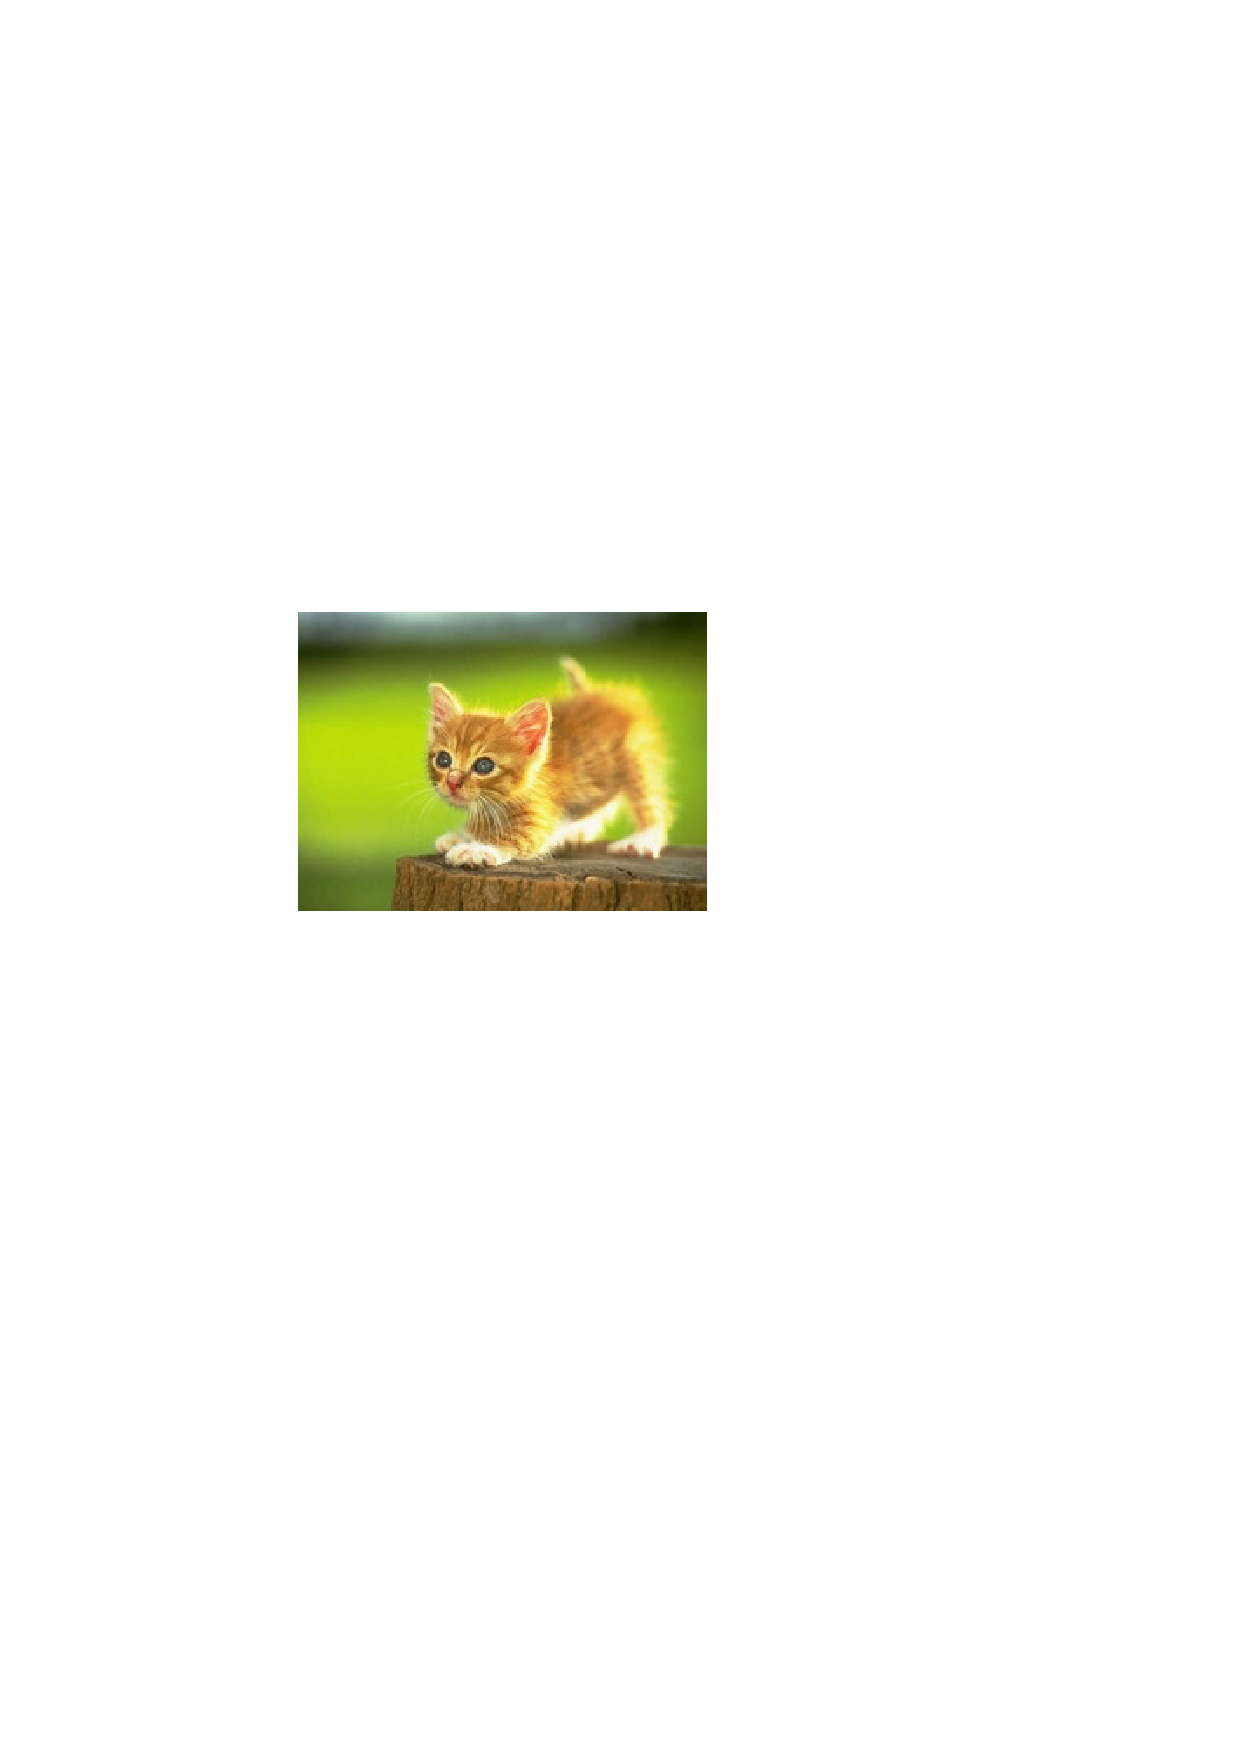
\includegraphics[width=\textwidth]{fig-example.pdf}
%   \caption{图片1}\label{fig:2-1}
%   \end{subfigure}
%   ~
%   \begin{subfigure}[b]{0.3\textwidth}
%   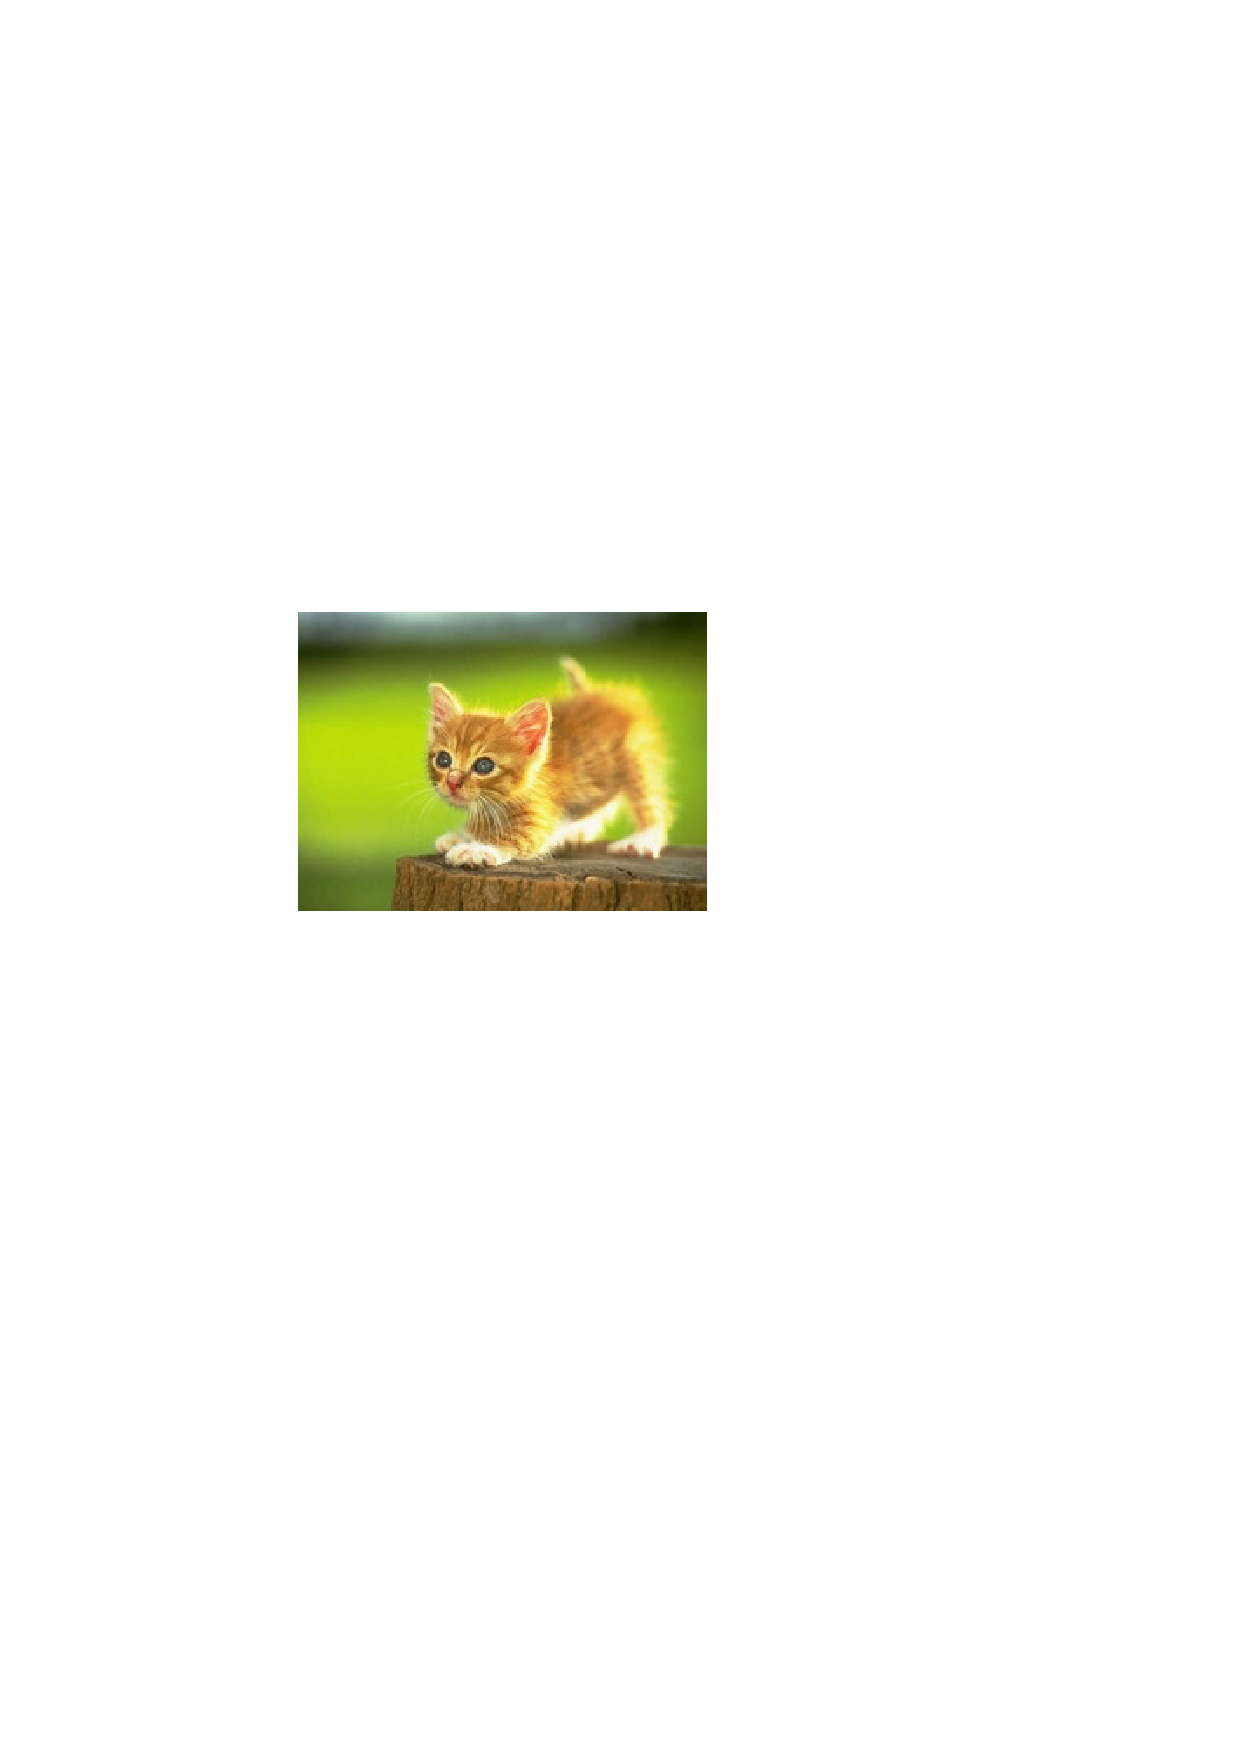
\includegraphics[width=\textwidth]{fig-example.pdf}
%   \caption{图片2}\label{fig:2-2}
%   \end{subfigure}
% \caption{多个图片}\label{fig:2}
% \end{figure}


\backmatter


\bibliography{ref-research}

\appendix

% \begin{publications}
%     \item 论文1
%     \item 论文2
% \end{publications}
\clearpage
\phantomsection
\chapter*{个人简历}
\addcontentsline{toc}{chapter}{\quad{}个人简历}
% 附录正文。




\end{document}
% \endinput
%%
%% End of file `hustreport-zh-example.tex'.
